% Bagian Hasil Percobaan
\section*{Hasil Percobaan} % Jika ada hasil percobaan

Hasil percobaan yang diperoleh adalah sebagai berikut:

\subsection*{Percobaan 1: Konfigurasi Static Routing}

\begin{itemize}
    \item \textbf{Konfigurasi Router 1}
    \begin{figure} [H]
        \centering
        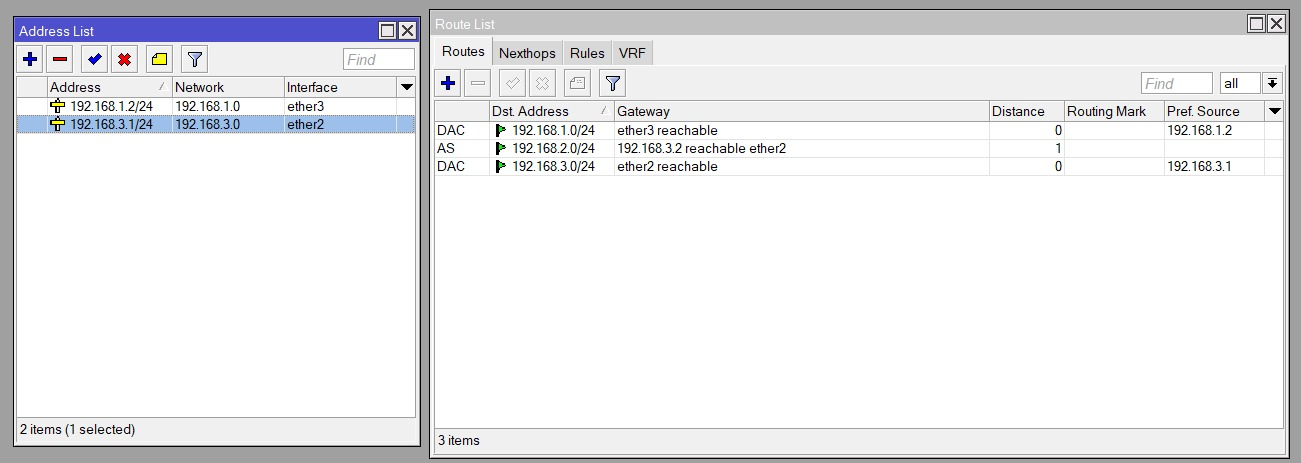
\includegraphics[width=0.8\textwidth]{img/percobaan 1_1_config.jpeg}
        \caption{Konfigurasi Router 1}
        \label{fig:router1}
    \end{figure}

    \item \textbf{Konfigurasi Router 2}
    \begin{figure} [H]
        \centering
        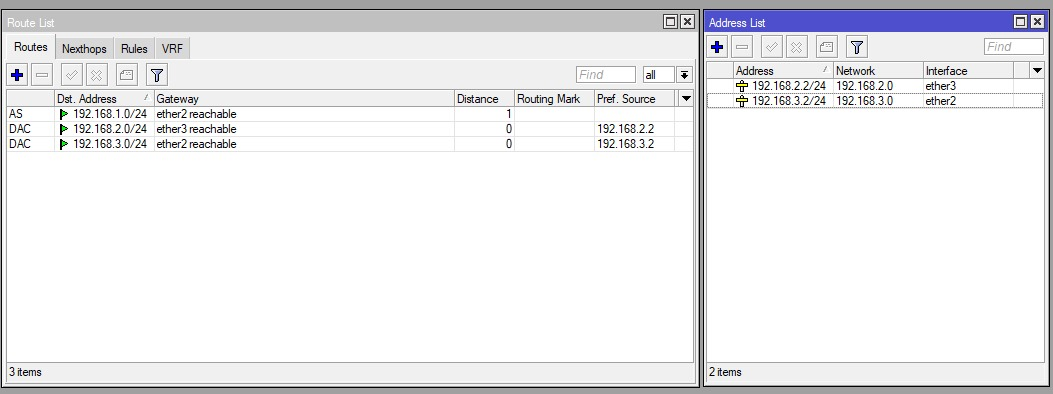
\includegraphics[width=0.8\textwidth]{img/percobaan 1_2_config.jpeg}
        \caption{Konfigurasi Router 2}
        \label{fig:router2}
    \end{figure}

    \item \textbf{Pengujian Pada Router 1 ke Router 2}
    \begin{figure} [H]
        \centering
        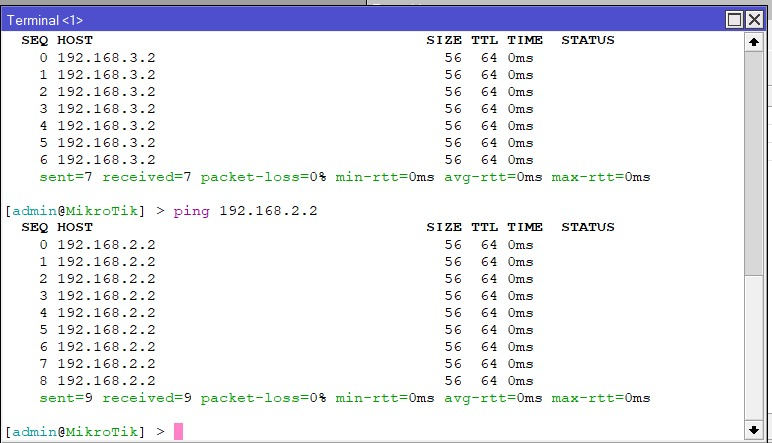
\includegraphics[width=0.8\textwidth]{img/percobaan 1_1_hasil.jpeg}
        \caption{Pengujian Pada Router 1}
        \label{fig:ping1}
    \end{figure}

    \item \textbf{Pengujian Pada Router 2 ke Router 1}
    \begin{figure} [H]
        \centering
        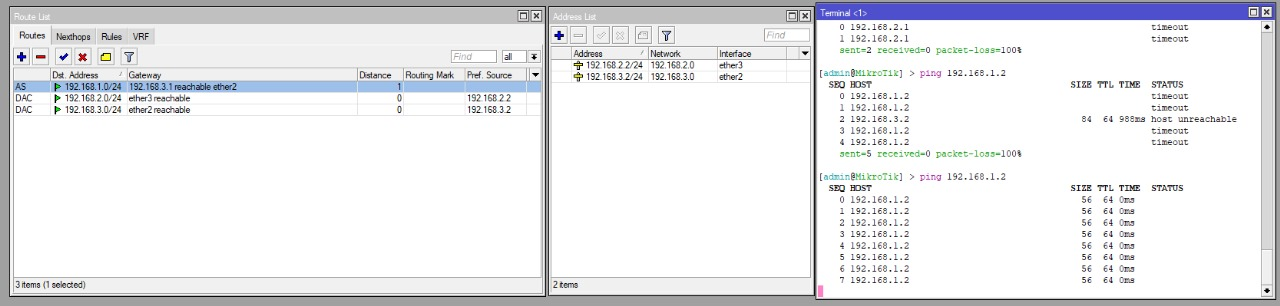
\includegraphics[width=0.8\textwidth]{img/percobaan 1_2_hasil.jpeg}
        \caption{Pengujian Pada Router 2}
        \label{fig:ping2}
    \end{figure}
\end{itemize}

\subsection*{Percobaan 2: Konfigurasi Dynamic Routing}

\begin{itemize}
    \item \textbf{Konfigurasi Router 1}
    \begin{figure} [H]
        \centering
        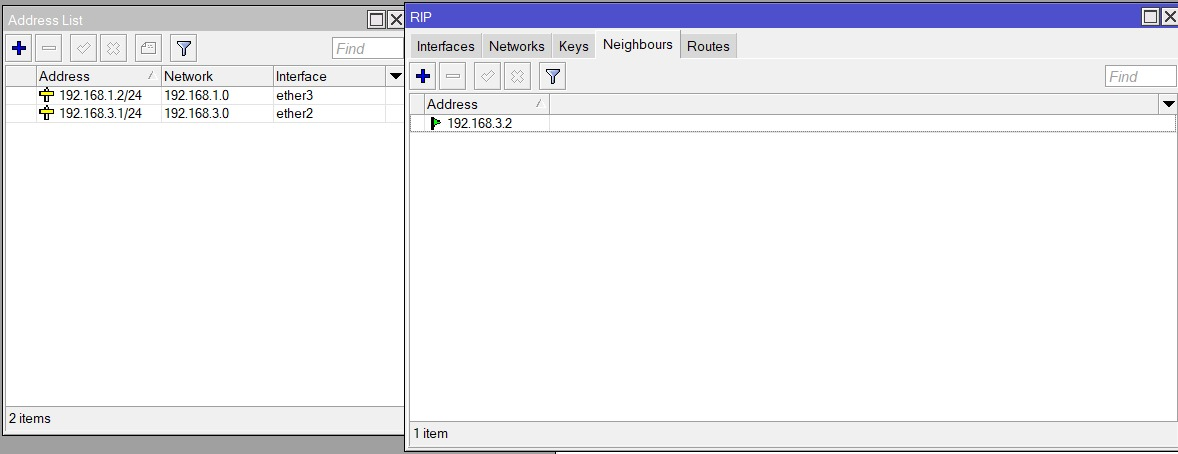
\includegraphics[width=0.8\textwidth]{img/percobaan 2_1_config.jpeg}
        \caption{Konfigurasi Router 1}
        \label{fig:router1_2}
    \end{figure}

    
    \item \textbf{Pengujian Pada Router 1 ke Router 2}
    \begin{figure} [H]
        \centering
        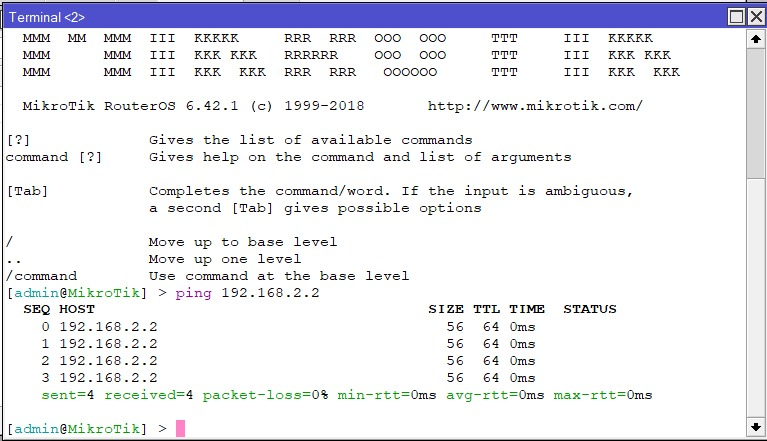
\includegraphics[width=0.8\textwidth]{img/percobaan 2_1_hasil.jpeg}
        \caption{Pengujian Pada Router 1}
        \label{fig:ping1_2}
    \end{figure}

    \item \textbf{Konfigurasi Router 2 dan Pengujian}
    \begin{figure} [H]
        \centering
        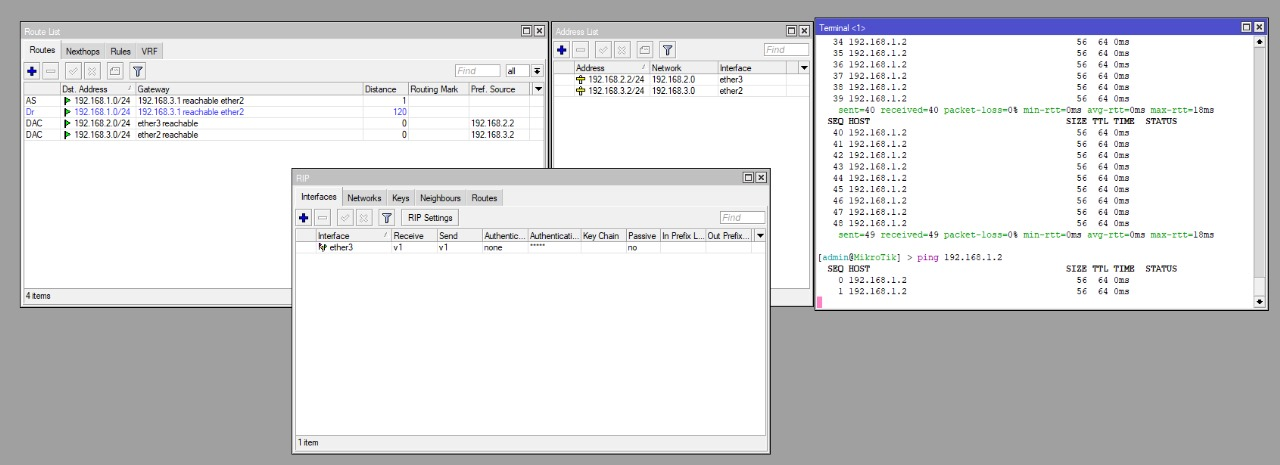
\includegraphics[width=1\textwidth]{img/percobaan 2_2.jpeg}
        \caption{Konfigurasi dan Hasil Pengujian Router 2}
        \label{fig:router2_2}
    \end{figure}
\end{itemize}

